\section{Digitaltechnik 1}
\subsection{Wahrheitstabelle, KDNF, KKNF, Y-Diagramm}
\begin{tabular}{ll}
  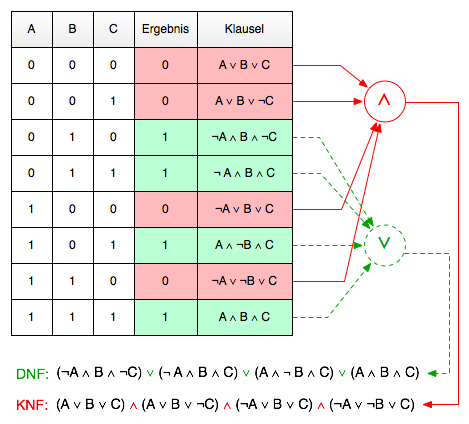
\includegraphics[width=0.3\textwidth]{pics/KNFDNF} & 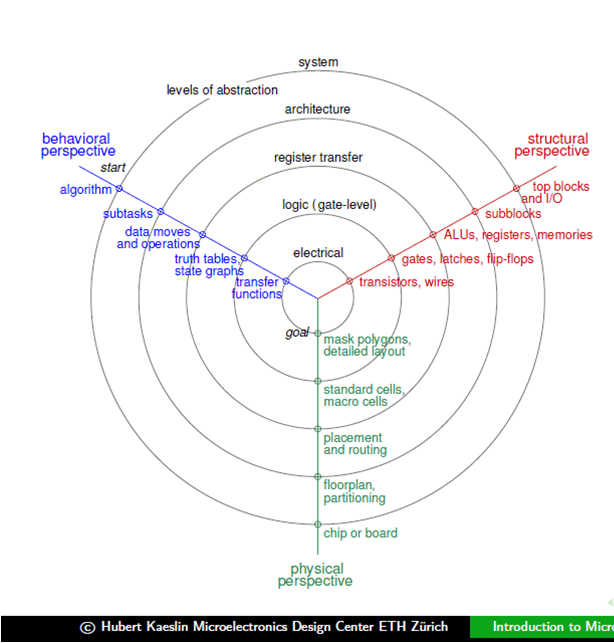
\includegraphics[width=0.3\textwidth]{pics/ydiagramm} \\
\end{tabular}
Kurzschreibweisen:\\
KNF: $ a = \&([1],[2],3) $ \\
DNF: $ b = \#([1],[3],37) $ \\
Zeugs in eckigen Klammern bedeutet don't care.
\subsection{Karnaugh-Diagramm}
\begin{tabular}{lll}
  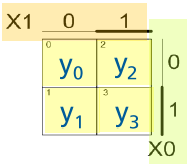
\includegraphics[width=0.1\textwidth]{pics/kv/2erKV} & 
  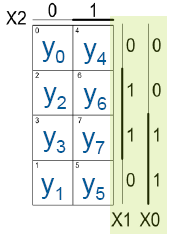
\includegraphics[width=0.1\textwidth]{pics/kv/3erKV} &
  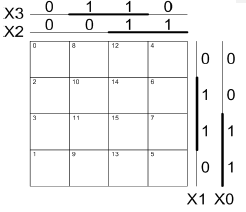
\includegraphics[width=0.2\textwidth]{pics/kv/4erKV}\\
\end{tabular}
\subsection{Arbeiten mit KV-Diagramm}
\begin{enumerate}
\setlength{\itemsep}{1pt}
  \setlength{\parskip}{0pt}
  \setlength{\parsep}{0pt}
\item Aufstellen der Wahrheitstabelle.\\
\item "Ubertragen der Werte der Wahrheitstabelle in KV Diagramm.\\
\item M"oglichst grosse Gruppen a $2^n$ Felder bilden.\\
\item
\begin{tabular}{ll}
  DNF & KNF \\
  Gruppen von Feldern mit Wert 1 oder d & Gruppen von Feldern mit Wert 0 oder d\\
  Primimplikanten: AND Verkn. & Primimplikanten: OR Verkn.\\
  OR Verkn. aller Primimpl. & AND Verkn. aller Primimpl.\\
\end{tabular}
\end{enumerate}